\documentclass[11pt,a4paper,notitlepage]{report}
% Shared preamble for the raw chapter-4 write-ups under docs/report/insights/.
%
% Each experiment_N/experiment_N.tex is a standalone, compilable LaTeX report
% written BEFORE anything goes into final_report/chapters/chapter_4_*.tex.
% It uses the final report's fonts, units and macros so that passages, tables
% and figures lift into the chapter without reformatting.
%
%   \documentclass[11pt,a4paper]{report}
%   % Shared preamble for the raw chapter-4 write-ups under docs/report/insights/.
%
% Each experiment_N/experiment_N.tex is a standalone, compilable LaTeX report
% written BEFORE anything goes into final_report/chapters/chapter_4_*.tex.
% It uses the final report's fonts, units and macros so that passages, tables
% and figures lift into the chapter without reformatting.
%
%   \documentclass[11pt,a4paper]{report}
%   % Shared preamble for the raw chapter-4 write-ups under docs/report/insights/.
%
% Each experiment_N/experiment_N.tex is a standalone, compilable LaTeX report
% written BEFORE anything goes into final_report/chapters/chapter_4_*.tex.
% It uses the final report's fonts, units and macros so that passages, tables
% and figures lift into the chapter without reformatting.
%
%   \documentclass[11pt,a4paper]{report}
%   \input{../common/preamble}
%   \begin{document} ...
%
% Figures and tables are NOT copied: \graphicspath and \reporttable resolve into
% final_report/figures/ and final_report/tables/, so the raw write-up always
% shows the same artefacts as the chapter.  Compile with:  latexmk -pdf <file>

\usepackage[T1]{fontenc}
\usepackage[utf8]{inputenc}
\usepackage{mathptmx}
\usepackage[scaled=0.92]{helvet}
\usepackage{courier}
\usepackage[a4paper,left=30mm,right=20mm,top=25mm,bottom=25mm]{geometry}
\usepackage{microtype}
\usepackage{booktabs}
\usepackage{tabularx}
\usepackage{longtable}
\usepackage{array}
\usepackage{multirow}
\usepackage{amsmath}
\usepackage{amssymb}
\usepackage{ifthen}
\usepackage{siunitx}
\usepackage{graphicx}
\usepackage{placeins}
\usepackage{caption}
\usepackage{enumitem}
\usepackage[table]{xcolor}
\usepackage{rotating}
\PassOptionsToPackage{hyphens}{url}\usepackage{url}
\usepackage[hidelinks]{hyperref}
\usepackage[nameinlink,noabbrev]{cleveref}

\graphicspath{{../../final_report/}{../../final_report/figures/}}
% \reporttable{name} inputs final_report/tables/name.tex
\newcommand{\reporttable}[1]{\input{../../final_report/tables/#1}}

\newcommand{\repo}[1]{\texttt{\detokenize{#1}}}
\sisetup{detect-all,group-separator={,},range-phrase=--,range-units=single}
\DeclareSIUnit{\pixel}{px}
\DeclareSIUnit{\mebi}{Mi}
\captionsetup{font=small,labelfont=bf}
\setlist{nosep}
\setlength{\parskip}{4pt}
\setlength{\LTcapwidth}{\textwidth}

% ---- result-slot status (RENDERED here, unlike in the final report)
\definecolor{stcompleted}{HTML}{A5D6A7}
\definecolor{stpartial}{HTML}{FFF2CC}
\definecolor{stuntested}{HTML}{FFD8A8}
\definecolor{stblocked}{HTML}{FFCDD2}
\definecolor{stfailed}{HTML}{FFCDD2}
\definecolor{stplanned}{HTML}{E0E0E0}
\newcommand{\slotstatus}[2]{%
  \par\noindent\fcolorbox{black!40}{st#1}{\parbox{\dimexpr\textwidth-2\fboxsep-2\fboxrule}{%
    \textbf{Status: #1.}\ #2}}\par\medskip}
\newcommand{\status}[1]{\textbf{#1}}

% ---- queries: RENDERED in red here so a reader sees every open concern in place
\definecolor{flagred}{HTML}{B00000}
\newcommand{\flag}[1]{\textcolor{flagred}{#1}}
\newcommand{\moved}[1]{#1}
\newenvironment{queried}[1][Questionable]%
  {\par\addvspace{0.6ex}\begingroup\color{flagred}\noindent
   \textbf{[#1]}\ \ignorespaces}%
  {\par\endgroup\addvspace{0.6ex}}

% ---- per-block performance marks (section 4.5 diagrams)
\definecolor{perfgood}{HTML}{A5D6A7}
\definecolor{perfpoor}{HTML}{FFCDD2}
\definecolor{perfnoeffect}{HTML}{D9EAF7}
\definecolor{perfnone}{HTML}{FFF2CC}
\newcommand{\perfmark}[1]{%
  \ifthenelse{\equal{#1}{good}}{\colorbox{perfgood}{\scriptsize good}}{%
  \ifthenelse{\equal{#1}{poor}}{\colorbox{perfpoor}{\scriptsize poor}}{%
  \ifthenelse{\equal{#1}{noeffect}}{\colorbox{perfnoeffect}{\scriptsize no effect}}{%
  \colorbox{perfnone}{\scriptsize no claim}}}}}

%   \begin{document} ...
%
% Figures and tables are NOT copied: \graphicspath and \reporttable resolve into
% final_report/figures/ and final_report/tables/, so the raw write-up always
% shows the same artefacts as the chapter.  Compile with:  latexmk -pdf <file>

\usepackage[T1]{fontenc}
\usepackage[utf8]{inputenc}
\usepackage{mathptmx}
\usepackage[scaled=0.92]{helvet}
\usepackage{courier}
\usepackage[a4paper,left=30mm,right=20mm,top=25mm,bottom=25mm]{geometry}
\usepackage{microtype}
\usepackage{booktabs}
\usepackage{tabularx}
\usepackage{longtable}
\usepackage{array}
\usepackage{multirow}
\usepackage{amsmath}
\usepackage{amssymb}
\usepackage{ifthen}
\usepackage{siunitx}
\usepackage{graphicx}
\usepackage{placeins}
\usepackage{caption}
\usepackage{enumitem}
\usepackage[table]{xcolor}
\usepackage{rotating}
\PassOptionsToPackage{hyphens}{url}\usepackage{url}
\usepackage[hidelinks]{hyperref}
\usepackage[nameinlink,noabbrev]{cleveref}

\graphicspath{{../../final_report/}{../../final_report/figures/}}
% \reporttable{name} inputs final_report/tables/name.tex
\newcommand{\reporttable}[1]{\input{../../final_report/tables/#1}}

\newcommand{\repo}[1]{\texttt{\detokenize{#1}}}
\sisetup{detect-all,group-separator={,},range-phrase=--,range-units=single}
\DeclareSIUnit{\pixel}{px}
\DeclareSIUnit{\mebi}{Mi}
\captionsetup{font=small,labelfont=bf}
\setlist{nosep}
\setlength{\parskip}{4pt}
\setlength{\LTcapwidth}{\textwidth}

% ---- result-slot status (RENDERED here, unlike in the final report)
\definecolor{stcompleted}{HTML}{A5D6A7}
\definecolor{stpartial}{HTML}{FFF2CC}
\definecolor{stuntested}{HTML}{FFD8A8}
\definecolor{stblocked}{HTML}{FFCDD2}
\definecolor{stfailed}{HTML}{FFCDD2}
\definecolor{stplanned}{HTML}{E0E0E0}
\newcommand{\slotstatus}[2]{%
  \par\noindent\fcolorbox{black!40}{st#1}{\parbox{\dimexpr\textwidth-2\fboxsep-2\fboxrule}{%
    \textbf{Status: #1.}\ #2}}\par\medskip}
\newcommand{\status}[1]{\textbf{#1}}

% ---- queries: RENDERED in red here so a reader sees every open concern in place
\definecolor{flagred}{HTML}{B00000}
\newcommand{\flag}[1]{\textcolor{flagred}{#1}}
\newcommand{\moved}[1]{#1}
\newenvironment{queried}[1][Questionable]%
  {\par\addvspace{0.6ex}\begingroup\color{flagred}\noindent
   \textbf{[#1]}\ \ignorespaces}%
  {\par\endgroup\addvspace{0.6ex}}

% ---- per-block performance marks (section 4.5 diagrams)
\definecolor{perfgood}{HTML}{A5D6A7}
\definecolor{perfpoor}{HTML}{FFCDD2}
\definecolor{perfnoeffect}{HTML}{D9EAF7}
\definecolor{perfnone}{HTML}{FFF2CC}
\newcommand{\perfmark}[1]{%
  \ifthenelse{\equal{#1}{good}}{\colorbox{perfgood}{\scriptsize good}}{%
  \ifthenelse{\equal{#1}{poor}}{\colorbox{perfpoor}{\scriptsize poor}}{%
  \ifthenelse{\equal{#1}{noeffect}}{\colorbox{perfnoeffect}{\scriptsize no effect}}{%
  \colorbox{perfnone}{\scriptsize no claim}}}}}

%   \begin{document} ...
%
% Figures and tables are NOT copied: \graphicspath and \reporttable resolve into
% final_report/figures/ and final_report/tables/, so the raw write-up always
% shows the same artefacts as the chapter.  Compile with:  latexmk -pdf <file>

\usepackage[T1]{fontenc}
\usepackage[utf8]{inputenc}
\usepackage{mathptmx}
\usepackage[scaled=0.92]{helvet}
\usepackage{courier}
\usepackage[a4paper,left=30mm,right=20mm,top=25mm,bottom=25mm]{geometry}
\usepackage{microtype}
\usepackage{booktabs}
\usepackage{tabularx}
\usepackage{longtable}
\usepackage{array}
\usepackage{multirow}
\usepackage{amsmath}
\usepackage{amssymb}
\usepackage{ifthen}
\usepackage{siunitx}
\usepackage{graphicx}
\usepackage{placeins}
\usepackage{caption}
\usepackage{enumitem}
\usepackage[table]{xcolor}
\usepackage{rotating}
\PassOptionsToPackage{hyphens}{url}\usepackage{url}
\usepackage[hidelinks]{hyperref}
\usepackage[nameinlink,noabbrev]{cleveref}

\graphicspath{{../../final_report/}{../../final_report/figures/}}
% \reporttable{name} inputs final_report/tables/name.tex
\newcommand{\reporttable}[1]{\input{../../final_report/tables/#1}}

\newcommand{\repo}[1]{\texttt{\detokenize{#1}}}
\sisetup{detect-all,group-separator={,},range-phrase=--,range-units=single}
\DeclareSIUnit{\pixel}{px}
\DeclareSIUnit{\mebi}{Mi}
\captionsetup{font=small,labelfont=bf}
\setlist{nosep}
\setlength{\parskip}{4pt}
\setlength{\LTcapwidth}{\textwidth}

% ---- result-slot status (RENDERED here, unlike in the final report)
\definecolor{stcompleted}{HTML}{A5D6A7}
\definecolor{stpartial}{HTML}{FFF2CC}
\definecolor{stuntested}{HTML}{FFD8A8}
\definecolor{stblocked}{HTML}{FFCDD2}
\definecolor{stfailed}{HTML}{FFCDD2}
\definecolor{stplanned}{HTML}{E0E0E0}
\newcommand{\slotstatus}[2]{%
  \par\noindent\fcolorbox{black!40}{st#1}{\parbox{\dimexpr\textwidth-2\fboxsep-2\fboxrule}{%
    \textbf{Status: #1.}\ #2}}\par\medskip}
\newcommand{\status}[1]{\textbf{#1}}

% ---- queries: RENDERED in red here so a reader sees every open concern in place
\definecolor{flagred}{HTML}{B00000}
\newcommand{\flag}[1]{\textcolor{flagred}{#1}}
\newcommand{\moved}[1]{#1}
\newenvironment{queried}[1][Questionable]%
  {\par\addvspace{0.6ex}\begingroup\color{flagred}\noindent
   \textbf{[#1]}\ \ignorespaces}%
  {\par\endgroup\addvspace{0.6ex}}

% ---- per-block performance marks (section 4.5 diagrams)
\definecolor{perfgood}{HTML}{A5D6A7}
\definecolor{perfpoor}{HTML}{FFCDD2}
\definecolor{perfnoeffect}{HTML}{D9EAF7}
\definecolor{perfnone}{HTML}{FFF2CC}
\newcommand{\perfmark}[1]{%
  \ifthenelse{\equal{#1}{good}}{\colorbox{perfgood}{\scriptsize good}}{%
  \ifthenelse{\equal{#1}{poor}}{\colorbox{perfpoor}{\scriptsize poor}}{%
  \ifthenelse{\equal{#1}{noeffect}}{\colorbox{perfnoeffect}{\scriptsize no effect}}{%
  \colorbox{perfnone}{\scriptsize no claim}}}}}

\usepackage{pgfplots}
\pgfplotsset{compat=1.17}
\renewcommand{\bibname}{References}
\setcounter{chapter}{3}
\renewcommand{\thesection}{\arabic{section}}
\renewcommand{\thefigure}{G.\arabic{figure}}
\renewcommand{\thetable}{G.\arabic{table}}
\title{GPU Acceleration of the ORB-SLAM3 Front End\\
       \large Engineering note for Chapter 3 (implemented system), with its validation measurements}
\author{Bolton Athit Davies}
\date{Reporting cutoff: 29 October 2026; revised 3 November 2026}
\begin{document}
\maketitle

\noindent\textbf{Purpose of this document.} This note records what was changed
in the ORB-SLAM3 fork to move its feature front end onto the GPU, how the change
was validated, and what the validation runs revealed. It is written for
Chapter~3 (the implemented system and its planned-versus-implemented table) and
for the threats-to-validity discussion of Chapter~4. It is not a result slot:
no Chapter~4 result uses this code yet, and the simulation configurations are
unchanged. Every number traces to a file under \repo{output/compare/real/}
named in \cref{sec:gpu-rules}.

\slotstatus{completed}{Implemented and validated on the laptop (RTX~3070) for
the real-rig configuration: extractor patch (10) and stereo-matcher patch
(10b), enabled by default in \repo{orbslam3_ros2/config/wil/stereo*.yaml}; a
pre-existing relocalisation crash found during validation is fixed (patch 11), and
the validation of this and the following days found five more out-of-bounds reads,
an Eigen temporary read after its scope and a layout mismatch between node and
library, all fixed (patches 12 to 14b, node build flag); an AddressSanitizer run
over a whole real recording is clean. The stereo-inertial mode, which shares this
front end, reached a reproducible \SI{0.48}{\metre} on \repo{dataset_realv6_000}
on 3 November (\cref{sec:gpu-inertial}). Portability to the Jetson platform is
\status{untested}. The fork changes are not yet committed.}

% =====================================================================
\section{Why the front end was moved}
\label{sec:gpu-why}

On the real rig the tracker could not keep up with the camera: it took about
\SI{85}{\milli\second} per stereo pair against a \SI{33}{\milli\second} frame
period, so two frames in three were dropped. Roughly \SI{80}{\percent} of that
time was ORB extraction \cite{rublee2011}, one CPU thread per camera computing
FAST \cite{rosten2006} on an eight-level pyramid of a
\num{1920}\(\times\)\num{1080} fisheye image, then the rotated BRIEF
descriptor \cite{calonder2010}. Dropped frames are not a uniform loss: they
cluster in turns, where inter-frame motion is largest, which is where the
real-rig trajectories were observed to fail.

The remaining cost after extraction was the stereo matcher. ORB-SLAM3
\cite{campos2021} matches the two fisheye views by brute force over every
descriptor pair inside the lapping area, which on this rig is the full image
width, so about \num{2000}\(\times\)\num{2000} Hamming distances are computed
per frame. \Cref{tab:gpu-stages} gives the stage split measured in isolation
on two recorded frame pairs.

\begin{table}[htbp]
\centering
\caption{Time per stereo frame of the fisheye stereo front end, measured in a
standalone harness on two \repo{dataset_realv5_000} frame pairs
(\num{1920}\(\times\)\num{1080}, \num{2000} features per camera, 8 levels).
Mean of 10 repetitions after a warm-up. The CPU matcher figure is with all 16
hardware threads idle; single-threaded it is \SI{38.2}{\milli\second}.}
\label{tab:gpu-stages}
\small
\begin{tabular}{lrrr}
\toprule
Stage & CPU & GPU extractor & GPU extractor + matcher \\
 & (\si{\milli\second}) & (\si{\milli\second}) & (\si{\milli\second}) \\
\midrule
Extraction, both cameras (two threads) & 41.8 & 12.1 & 12.1 \\
Brute-force Hamming 2-NN matching       &  9.2 &  8.2 &  0.44 \\
Ratio test                              &  0.1 &  0.1 &  0.1 \\
Triangulation of accepted matches       &  0.2 &  0.2 &  0.2 \\
\midrule
Sum                                     & 51.3 & 20.6 & 12.8 \\
\bottomrule
\end{tabular}
\end{table}

% =====================================================================
\section{What moved and what did not}
\label{sec:gpu-design}

The per-pixel and per-keypoint arithmetic moved; the selection logic stayed.
On the GPU: the FAST-9 corner score (a literal port of OpenCV's
\texttt{cornerScore<16>}), non-maximum suppression with ORB-SLAM3's
two-threshold cell rule, the \(7\times7\) Gaussian blur, the intensity-centroid
orientation and the rotated BRIEF descriptor; since patch (10b) also the
brute-force Hamming 2-nearest-neighbour stereo matching. On the CPU, unchanged:
the image pyramid, the dynamic-object mask veto used by the Experiment~3
filter, the octree keypoint distribution that gives ORB-SLAM3 its uniform
coverage, and everything downstream of the frame.

Keeping the selection on the CPU is what makes the output comparable. The GPU
produces the same candidate set and the same scores, and the stock
distribution picks from them, so a frame extracted on the GPU is the frame
ORB-SLAM3 would have extracted, up to tie-breaks between corners of equal
score (\cref{sec:gpu-fidelity}). The fisheye camera model
\cite{kannala2006} and the pinhole stereo path are untouched, so the
simulation configurations, which keep the switch off, run the stock code.

No CUDA toolkit is needed to build the fork. The driver library and the NVRTC
runtime compiler \cite{nvidia2026nvrtc} are loaded with \texttt{dlopen} on
first use and the kernels are compiled from a source string at start-up, once
per process (about \SI{90}{\milli\second}). If any step fails, the extractor
logs one line and runs the CPU path. \Cref{tab:gpu-keys} lists the three
settings that control the path.

\begin{table}[htbp]
\centering
\caption{Settings that control the GPU front end. Both real-rig configurations
set \texttt{ORBextractor.useGPU: 1}; both simulation configurations omit it.}
\label{tab:gpu-keys}
\small
\begin{tabularx}{\textwidth}{lX}
\toprule
Setting & Meaning \\
\midrule
\texttt{ORBextractor.useGPU} (YAML, 0/1) & GPU extraction; absent = 0. \\
\texttt{Stereo.useGPUMatch} (YAML, 0/1) & GPU stereo matching; absent = follow \texttt{useGPU}. Used only for A/B runs. \\
\texttt{ORB\_SLAM3\_NVRTC\_DIR} (environment) & Directory of \texttt{libnvrtc.so.12} when it is not on the loader path. \\
\bottomrule
\end{tabularx}
\end{table}

% =====================================================================
\section{Validation}
\label{sec:gpu-validation}

\subsection{Fidelity of the GPU extractor}
\label{sec:gpu-fidelity}

The GPU extractor reproduces the CPU extractor to within tie-breaks.
\Cref{tab:gpu-fidelity} compares the two on four recorded frames: nine in ten
GPU keypoints sit at the identical pixel and octave of a CPU keypoint, and on
those the orientation is equal and the descriptors differ by a third of a bit
on average. The remaining tenth are corners of equal FAST score that the
GPU's suppression order and the octree resolve differently; they are not a
different detector.

\begin{table}[htbp]
\centering
\caption{CPU versus GPU extractor on four \repo{dataset_realv5_000} frames
(\num{1920}\(\times\)\num{1080}, \num{2000} features, 8 levels, RTX~3070).
``Identical'' means the same pixel position and octave; the descriptor
comparison is over those keypoints. Time is the mean of 15 repetitions.}
\label{tab:gpu-fidelity}
\small
\begin{tabular}{lr}
\toprule
Quantity & Value \\
\midrule
Time per image, CPU & \SI{39}{\milli\second} \\
Time per image, GPU & \SI{9.3}{\milli\second} \\
Keypoints per level, difference & \(\pm 2\) \\
GPU keypoints identical to a CPU keypoint & \SI{90}{\percent} \\
Orientation difference on identical keypoints & \SI{0.00}{\degree} \\
Descriptor Hamming distance on identical keypoints, mean & \num{0.35} bits \\
Descriptors bit-identical / within 2 bits & \SI{73}{\percent} / \SI{99}{\percent} \\
\bottomrule
\end{tabular}
\end{table}

\subsection{Fidelity of the GPU stereo matcher}

The GPU matcher is exact. On the two frame pairs of \cref{tab:gpu-stages} it
returned, for every one of the \num{2003} and \num{2005} query descriptors,
the same best index and the same two distances as OpenCV's brute-force
matcher, including its tie order, so the ratio test downstream accepted the
identical sets (\num{391} and \num{387} matches). Its cost is
\SI{0.44}{\milli\second} per frame against \SIrange{8.2}{10.0}{\milli\second}.

\subsection{Effect inside the running node}
\label{sec:gpu-node}

In the node the gain is smaller than the harness suggests, because the
stages that remain on the CPU become the larger share. \Cref{tab:gpu-abba}
reports the controlled comparison for the stereo matcher: the tracker falls
from \SI{64}{\milli\second} to \SI{45}{\milli\second} per frame at real-time
replay, \SI{35}{\percent} more frames are processed, and the inlier and
map-point counts are unchanged. The two runs of each arm agree to within
\SI{1}{\milli\second}. \Cref{fig:gpu-stages} shows where the remaining
\SI{45}{\milli\second} go; it is still above the frame period, so frames
still drop at \SI{30}{\hertz}, fewer than before.

\begin{table}[htbp]
\centering
\caption{Node A/B of the stereo matcher on \repo{dataset_realv5_000}, first
\SI{60}{\second} of the recording, stereo-only, loop closing off, viewer off,
ABBA order, each run started with the CPU package below \SI{75}{\celsius}.
Both arms use the GPU extractor. Medians over frames in the tracking-OK state.
Source: \repo{output/compare/real/gpu-stereo-matcher-ab/gpu_match_abba_metrics.csv}.}
\label{tab:gpu-abba}
\small
\resizebox{\textwidth}{!}{%
\begin{tabular}{llrrrrrrr}
\toprule
Rate & Arm & Frames & Dropped & Extraction+stereo & Tracker total & Inliers & Map points & Losses \\
 & & processed & (\si{\percent}) & (\si{\milli\second}) & (\si{\milli\second}) & (median) & (final) & \\
\midrule
1.0 & A1 CPU matcher & 840  & 47 & 27.3 & 64.2 & 831 & 2498 & 0 \\
1.0 & B1 GPU matcher & 1153 & 34 & 14.8 & 44.7 & 851 & 2500 & 0 \\
1.0 & B2 GPU matcher & 1147 & 35 & 15.1 & 44.5 & 844 & 2444 & 0 \\
1.0 & A2 CPU matcher & 866  & 45 & 27.0 & 63.2 & 820 & 2711 & 0 \\
\midrule
0.5 & A1 CPU matcher & 1487 & 12 & 26.1 & 64.9 & 878 & 2734 & 0 \\
0.5 & B2 GPU matcher & 1660 &  7 & 14.4 & 50.1 & 917 & 2854 & 0 \\
0.5 & A2 CPU matcher (started at \SI{79}{\celsius}) & 1088 & 29 & 31.8 & 84.0 & 853 & 2883 & 0 \\
0.5 & B1 GPU matcher (started at \SI{95}{\celsius}) & 89 & -- & -- & -- & -- & -- & crashed, \cref{sec:gpu-defect} \\
\bottomrule
\end{tabular}}
\end{table}

\begin{figure}[htbp]
\centering
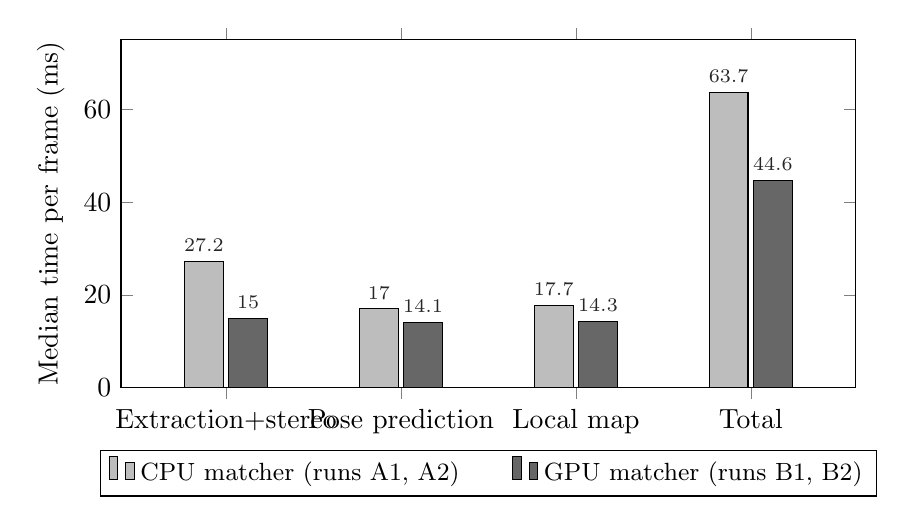
\begin{tikzpicture}
\begin{axis}[
  ybar, bar width=14pt, width=0.9\textwidth, height=6cm,
  ylabel={Median time per frame (ms)}, ymin=0, ymax=75,
  symbolic x coords={Extraction+stereo, Pose prediction, Local map, Total},
  xtick=data, enlarge x limits=0.2,
  legend style={at={(0.5,-0.18)}, anchor=north, legend columns=2, font=\small, /tikz/every even column/.append style={column sep=0.6cm}},
  nodes near coords, nodes near coords style={font=\scriptsize, color=black},
  every axis plot/.append style={fill opacity=0.85},
]
\addplot+[fill=black!30, draw=black] coordinates {(Extraction+stereo,27.2) (Pose prediction,17.0) (Local map,17.7) (Total,63.7)};
\addplot+[fill=black!70, draw=black] coordinates {(Extraction+stereo,15.0) (Pose prediction,14.1) (Local map,14.3) (Total,44.6)};
\legend{{CPU matcher (runs A1, A2)},{GPU matcher (runs B1, B2)}}
\end{axis}
\end{tikzpicture}
\caption{Tracker time per frame by stage, mean of the two runs per arm at
replay rate 1.0 from \cref{tab:gpu-abba} (\(n=2\) runs per arm, 840--1153
frames per run). The two CPU-side stages also fall by about
\SI{3}{\milli\second}: the CPU matcher launched a sixteen-thread parallel
loop on every frame that competed with the other threads. Data:
\repo{gpu_plugin_stage_means.csv} beside this note.}
\label{fig:gpu-stages}
\end{figure}

The extractor itself was compared in the node a day earlier without thermal
control (full recording, CPU arm then GPU arm back to back): tracker
\SIrange{110}{82}{\milli\second} at half speed and
\SIrange{206}{118}{\milli\second} at real time, frames processed
\SI{+23}{\percent} and \SI{+64}{\percent}, inliers and map points at parity,
no tracking loss in any run. The GPU arm ran second and still won, so the
direction is safe; the magnitudes are not controlled and are not quoted
further.

\subsection{A measurement condition found on the way}
\label{sec:gpu-thermal}

Back-to-back timing runs on this laptop are confounded by heat. In the first
matcher A/B, every run slowed from about \SI{60}{} to
\SI{150}{\milli\second} per frame as the CPU package passed
\SI{90}{\celsius} and throttled, so whichever arm ran second looked worse
regardless of code (\repo{order_confounded/} in the same directory). The
ABBA design with cool starts above was adopted in response, and the same
rule applies to every capacity table of Section~6.4 of the evaluation
protocol: start below \SI{75}{\celsius}, alternate arms, keep windows short,
and do not read effects under about \SI{20}{\percent} from full-recording
frame counts.

% =====================================================================
\section{A defect exposed by the validation runs}
\label{sec:gpu-defect}

Two validation runs ended in the segmentation fault that had been killing
real-rig runs after a tracking loss since the realv4 recordings
(``exit code \(-11\)''). Caught under a debugger, the fault is in the
relocalisation matcher of ORB-SLAM3, not in the GPU code. For a fisheye
camera the distortion vector handed to the frame is zero, so the
``undistorted'' keypoint list is a copy of the left-camera keypoints only,
while the keyframe's map-point list spans both cameras; a map point first
observed through the right camera indexes past the end of that list, the
resulting angle is not a number, and the orientation histogram is indexed
with \texttt{INT\_MIN}. Every other matcher routine on the tracking path
already guards this index; the relocalisation one did not, which is why the
crash appeared only on the fisheye rig and only after a loss.

The fix (patch 11) applies the same guard and keeps the original line as a
comment. On the patched library, forced relocalisations (a map built from the
first \SI{25}{\second}, then playback restarted at three other offsets, twice,
under the debugger) completed without a fault where the unpatched library
had crashed in four of the six runs that reached that path. Backtrace,
registers and the verification logs are under
\repo{output/compare/real/relocalisation-crash-patch11/}. For the report this
means every earlier real-rig run that lost tracking was cut short by this
defect rather than by the estimator's own recovery behaviour, and the
real-robot slots recorded after 29 October 2026 are the first on which a
tracking loss can be followed through.

% =====================================================================
\section{Stereo-inertial on the same recording}
\label{sec:gpu-inertial}

The inertial mode shares the GPU front end, and until this afternoon it did not
hold tracking on \repo{dataset_realv5_000} at all (ten map resets in thirty
seconds). The cause was not the front end. Three defects were found in order,
each by measurement, and \cref{tab:gpu-inertial} gives the run after each fix.

\begin{table}[htbp]
\centering
\caption{Stereo-inertial runs on \repo{dataset_realv5_000} at replay rate 0.5,
GPU front end on, loop closing on, one run per row. ``Starved'' frames are frames
skipped because fewer than two IMU samples had arrived for them. Source:
\repo{output/output_orb/real/realv5_imu_*/run_summary.csv}.}
\label{tab:gpu-inertial}
\small
\resizebox{\textwidth}{!}{%
\begin{tabular}{lrrrrrr}
\toprule
Configuration & IMU received & Starved & Resets & Loss events & Map points & Poses \\
\midrule
scale 1.0589 (old IMU), default buffers, first 30 s & 6370 & 146 & 10 & 30 & -- & 202 \\
scale 0.9923, default buffers & 22409 (83 \%) & 1063 & 19 & 73 & 3140 & 1060 \\
scale 0.9923, 64 MB socket buffers & 26813 (99.8 \%) & 615 & 19 & 78 & 177 & 1657 \\
\quad + IMU in its own callback group (reliable) & 26838 & \textbf{2} & \textbf{2} & 11 & \textbf{9768} & \textbf{2318} \\
\quad + IMU in its own group, best-effort & 26854 & 0 & 1 & 1 & 10068 & 1632 \\
\bottomrule
\end{tabular}}
\end{table}

\textbf{Accelerometer scale.} The launch file multiplied acceleration by 1.0589,
a correction measured on the previous (RealSense) IMU, which read \SI{9.26}{\metre\per\second\squared}
at rest. The rig's current IMU reads \SI{9.886}{\metre\per\second\squared} at rest
(stillest \SI{2}{\second} window of the recording, standard deviation 0.018), so
ORB-SLAM3 was fed \SI{10.47}{\metre\per\second\squared} against its fixed
\SI{9.81}{} and its inertial initialisation never converged. With the measured
factor, 0.9923, initialisation completed at \SI{3.2}{\second}.

\textbf{IMU delivery.} The IMU then arrived in bursts: zero messages between most
frames, then up to 1063 at once, while the image stream flowed one frame at a time,
so half of the frames were skipped for want of IMU data and the map reset on every
timestamp jump. Two layers were separated by two changes. Raising the kernel socket
buffers from the Linux default of \SI{208}{\kibi\byte} to \SI{64}{\mebi\byte}
stopped the loss (83 \% to 99.8 \% of messages delivered) but not the bursts.
Giving the IMU subscription its own reentrant callback group, so that it never
queues behind a JPEG decode in the node's default mutually exclusive group, removed
the bursts: starved frames 615 to 2, resets 19 to 2. A best-effort subscription was
added as a second lever and was not better (no starvation, but more dropped frames
and a slower tracker); the default stays reliable.

\textbf{What was left on 29 October, and what became of it.} The two remaining
resets at \SI{3.0}{} and \SI{5.6}{\second} are ORB-SLAM3's own IMU check during
initialisation; they appear in every inertial run since and are benign. The lever
arm was measured by tape that evening (left camera \SI{0.26}{\metre} above and
\SI{0.065}{\metre} in front of the IMU) and entered under the rotation already in
the file; the sign of the IMU's z axis and the lateral offset remain
\flag{unverified}. On \repo{dataset_realv6_000} the inertial mode then proved
unstable in a way none of this explained: identical runs scored between
\SI{0.4}{} and \SI{9.6}{\metre}. The resolution, documented in the engineering
record (sections 7.10 to 7.13) and in the Experiment 3 note, was that the
optimiser trusted an IMU whose axis signs, lever arm and time offset nobody had
verified; raising the configured IMU noise densities tenfold gave
\SI{0.49}{}, \SI{0.47}{} and \SI{0.49}{\metre} in three consecutive runs at
real-time replay, with the GPU front end on. Those three runs, not the
inertial rows of \cref{tab:gpu-inertial}, are the state of the inertial mode.

\flag{Resolution of these runs is not recorded in their manifests: the real-rig
inertial configuration carried \texttt{Camera.newWidth/newHeight} = 960/540 for part
of the afternoon (since commented out), so the inertial rows of
\cref{tab:gpu-inertial} may be at half resolution and are not comparable with
the stereo-only timings above.}

% =====================================================================
\section{Limitations and threats to validity}
\label{sec:gpu-threats}

\begin{itemize}
\item \textbf{Platform.} Validated on the development laptop (RTX~3070,
  driver 595) only. \flag{The real robot's Jetson Xavier NX has not been
  tried; its driver ships the same two libraries, but neither the runtime
  compilation nor the timings have been confirmed there.}
\item \textbf{Reproducibility.} GPU extraction is not bit-reproducible run to
  run, so repeated real-rig runs are statistical, as the simulation runs
  already are; the matcher is exact.
\item \textbf{Shared GPU.} In Experiment~3 the YOLO detector uses the same GPU.
  Contention between the detector and the front end was not measured.
\item \textbf{One recording.} All node measurements are on
  \repo{dataset_realv5_000}. The GPU timings are stereo-only; the stereo-inertial
  runs of \cref{sec:gpu-inertial} are counts of resets and starved frames, not
  timings, and their resolution is uncertain as flagged there.
\item \textbf{Configuration generation.} The real-rig configuration now
  differs from every earlier real recording's run (GPU front end, 28~October
  extrinsics, re-measured accelerometer scale, IMU callback group, measured
  lever arm). Earlier real-rig ORB-SLAM3 results are not repeats of it and are
  not pooled with it.
\item \textbf{Not yet committed.} The fork carries the patches of 29 October to
  3 November uncommitted, the ROS package its node, build-flag and configuration
  changes; run manifests cannot cite a commit for any of it until they are
  committed.
\end{itemize}

% =====================================================================
\section{Reporting rules}
\label{sec:gpu-rules}

Every number in this note traces to one of the following files.
\begin{itemize}
\item Harness measurements (\cref{tab:gpu-stages,tab:gpu-fidelity}): harness
  sources and the four frame images beside the A/B artefacts,\\
  \repo{output/compare/real/gpu-extractor-ab/gpu_orb_test.cc} and\\
  \repo{output/compare/real/gpu-stereo-matcher-ab/stereo_stage_test.cc}.
\item Node measurements (\cref{tab:gpu-abba,fig:gpu-stages}): per-run
  \repo{tracking_frontend.csv} and \repo{run_summary.csv}, the metrics table
  and the start/end temperatures, all under\\
  \repo{output/compare/real/gpu-stereo-matcher-ab/}.
\item Crash evidence (\cref{sec:gpu-defect}): backtraces, registers and the
  verification logs under\\
  \repo{output/compare/real/relocalisation-crash-patch11/}.
\item Stereo-inertial runs (\cref{tab:gpu-inertial}): \repo{run_summary.csv} and
  \repo{performance.csv} under\\
  \repo{output/output_orb/real/realv5_imu_*/} and, for the first row,\\
  \repo{~/output/wil_orbslam3_stereo_imu/}.
\item IMU rest value and arrival statistics: the bag itself and\\
  \repo{script/imu_arrival_probe.py}.
\item Engineering record: \repo{orbslam3_ros2/MEMORY_CLAUDE/integration.md},
  Sections~3.5, 3.5.1, 7.10 and 7.11.
\end{itemize}

\begin{thebibliography}{9}
\bibitem{rublee2011}
Rublee, E., Rabaud, V., Konolige, K. and Bradski, G., 2011, ``ORB: An Efficient Alternative to SIFT or SURF,'' \textbf{Proceedings of the IEEE International Conference on Computer Vision (ICCV 2011)}, 6--13 November 2011, Barcelona, Spain, pp.~2564--2571.
\bibitem{rosten2006}
Rosten, E. and Drummond, T., 2006, ``Machine Learning for High-Speed Corner Detection,'' \textbf{Computer Vision -- ECCV 2006, Lecture Notes in Computer Science, Vol. 3951}, 7--13 May 2006, Graz, Austria, pp.~430--443.
\bibitem{calonder2010}
Calonder, M., Lepetit, V., Strecha, C. and Fua, P., 2010, ``BRIEF: Binary Robust Independent Elementary Features,'' \textbf{Computer Vision -- ECCV 2010, Lecture Notes in Computer Science, Vol. 6314}, 5--11 September 2010, Heraklion, Greece, pp.~778--792.
\bibitem{campos2021}
Campos, C., Elvira, R., G\'omez Rodr\'iguez, J.J., Montiel, J.M.M. and Tard\'os, J.D., 2021, ``ORB-SLAM3: An Accurate Open-Source Library for Visual, Visual-Inertial, and Multi-Map SLAM,'' \textbf{IEEE Transactions on Robotics}, Vol.~37, No.~6, pp.~1874--1890.
\bibitem{kannala2006}
Kannala, J. and Brandt, S.S., 2006, ``A Generic Camera Model and Calibration Method for Conventional, Wide-Angle, and Fish-Eye Lenses,'' \textbf{IEEE Transactions on Pattern Analysis and Machine Intelligence}, Vol.~28, No.~8, pp.~1335--1340.
\bibitem{nvidia2026nvrtc}
NVIDIA Corporation, 2026, \textbf{NVRTC: CUDA Runtime Compilation User Guide} [Online], Available : \url{https://docs.nvidia.com/cuda/nvrtc/index.html} [2026, October 29].
\end{thebibliography}
\end{document}
